\documentclass[a4paper, 12pt]{report}

\usepackage{charter}
\usepackage{makeidx}
\usepackage{fancyhdr}
\usepackage{hyperref}
\usepackage[utf8]{inputenc}
\usepackage{graphicx}
\usepackage[left=2cm, right=2cm]{geometry}
\usepackage{latexsym}
\usepackage{amsmath, amsthm, amssymb}
\usepackage{rotating}


\begin{titlepage}
\title{Norme}
\author{Release 0.2}
\date{\today \\Firenze \\\begin{figure}[h] \centering 
\includegraphics[width=0.2\textwidth]{../images/logokiwi.png} \end{figure} }
\end{titlepage}

\pagestyle{fancy}

\begin{document}

\maketitle

\section*{Approvazione, redazione, lista distribuzione}
\begin{table}[h!]
  \begin{center}
    \begin{tabular}{| l | l | p{60mm} |}
    \hline
    \textbf{approvato da} & \textbf{il giorno} & \textbf{firma} \\
	\hline    
	Marco Tinacci & \today &  \\
    \hline
    \end{tabular}
  \end{center}
\end{table}

\begin{table}[h!]
  \begin{center}
    \begin{tabular}{| l | l | p{60mm} |}
    \hline
    \textbf{redatto da} & \textbf{il giorno} & \textbf{firma} \\
	\hline    
	Massimo Nocentini & \today &  \\
    \hline
    \end{tabular}
  \end{center}
\end{table}

\begin{table}[h!]
  \begin{center}
    \begin{tabular}{| l | l | p{60mm} |}
    \hline
    \textbf{distribuito a} & \textbf{il giorno} & \textbf{firma} \\
	\hline    
	Francesco Calabri & \today &  \\
    \hline
	Manuele Paulantonio & \today &  \\
    \hline
	Daniele Poggi & \today &  \\
    \hline
	Massimo Nocentini & \today &  \\
    \hline
	Niccol\'o Rogai & \today &  \\
    \hline
	Marco Tinacci & \today &  \\
    \hline
    \end{tabular}
  \end{center}
\end{table}

\tableofcontents

\newpage

\section{Introduzione}
Le norme di progetto sono divise in categorie (comunicazioni interne, documentazione, strumenti) e sotto categorie.

Nelle norme si avanza di major release sull'aggiunta di categorie significative mentre si avanza di minor per le modifiche e gli aggiornamenti minori di categorie e sotto categorie.

\section{Struttura del documento}

\chapter{Gestione del progetto}
\section{Modello di processo}
Come modello di riferimento usiamo il modello agile \textbf{ICONIX}, eventualmente adattando caso per caso le fasi principali.
\begin{figure}[h!] 
	\centering
	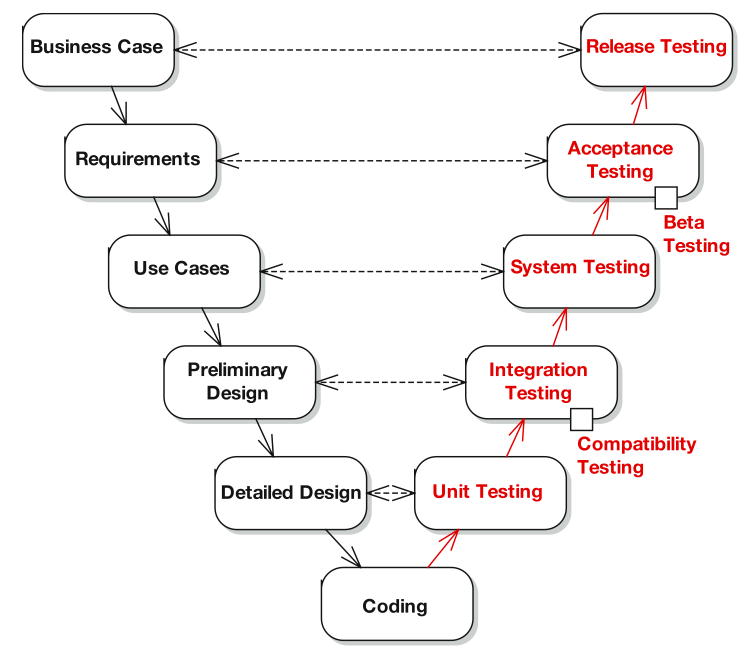
\includegraphics[width=1\textwidth]{gestione_progetto/vmodel.png}
	\caption{Modello a ``V'' che descrive le varie fasi di produzione e di testing}
	\label{fig:vModel} 
\end{figure}
La fase di analisi dei requisiti prevede la produzione dei documenti di domain model, use cases, metriche e mokup.
La fase di progettazione del sistema prevede la produzione dei diagrammi di sequenza e di classe, con descrizioni delle interfacce e degli algoritmi non banali.
La fase di progettazione delle prove prevede la produzione dei robustness diagrams al fine di produrre un documento contenente i test che si vogliono eseguire.

\chapter{Comunicazioni interne}
\section{Gruppo di discussione}
Ogni comunicazione rilevante riguardo al progetto deve essere comunicata sul gruppo di discussione \index{gruppo di discussione} all'indirizzo web \href{http://groups.google.it/group/kiwitp}{http://groups.google.it/group/kiwitp}  \index{gruppo di discussione!web site}. I componenti del gruppo sono tenuti a controllare frequentemente le comunicazioni, dopo 24 ore dalla pubblicazione della comunicazione si presuppone che questa sia stata letta. Se la scadenza ricade in un giorno festivo si assume che la comunicazione sia stata letta dopo il termine del primo giorno lavorativo successivo. 
Eventuali ritardi o impossibilità devono essere comunicati sempre sul gruppo con almeno 24 ore di anticipo sull'evento interessato.
Etichettare il titolo della discussione coi nomi delle persone interessate. Se la comunicazione è diretta a tutti i componenti del gruppo si può omettere i destinatari.


\chapter{Documentazione}
\section{Struttura delle directory e formato file}
Tutti i documenti risiedono in formato digitale (.tex) nella cartella \emph{"$/$documentazione\_progetto"} del server SVN del progetto (specificato negli strumenti usati). Definiamo la relazione fra tipi di modello e posizione nel file system:
\begin{description}
\item[diario] qui e' presente il file \emph{[Kiwi-MGC]diario.tex} che compone 
le informazioni divise nelle successive directory. Inoltre viene committato
anche il relativo \emph{[Kiwi-MGC]diario.pdf}, generato a partire dal file .tex,
 ogni volta che il file sorgente viene committato.
	\begin{description}
		\item[archivio]
		\item[consegne]
	\end{description}
\item[verbali] i file contenenti
	\begin{description}
		\item[riunioni\_committente] \quad
			\begin{description}
				\item[collaudo]
				\item[incontri\_analisi]
				\item[revisioni\_congiunte]	
			\end{description}
		\item[riunioni\_interne] \quad
			\begin{description}
				\item[collettive]
				\item[parziali]
			\end{description}
		\item[riunioni\_SQ]
	\end{description}
\item[norme] \quad
	\begin{description}
		\item[comunicazioni\_interne] \quad
		\item[documentazione]
		\item[strumenti]	
	\end{description}
\item[images]
\end{description}

\subsection{Sintassi valide esclusi i verbali}
I nomi dei file che non appartengono alle foglie della precedente struttura
devono rispettare la seguente sintassi: \\ 
$<$nome file$>$ ::= [$<$team$>$-$<$proj$>$]$<$file$>$.$<$ext$>$ \\
$<$file$>$ ::= organigramma | diario | norme | requisiti | offerta | disegno\_sistema | piano\_prove | prova\_$<$data$>$ \\
$<$ext$>$ ::= tex \\
$<$data$>$ ::= AAAAMMGG (anno su quattro cifre, mese e giorno su due cifre per
 far coincidere l'ordinsamento alfabetico con l'ordinamento cronologico) \\
$<$team$>$ ::= Kiwi\\
$<$proj$>$ ::= MGC

\subsection{Sintassi per i verbali}
nome della cartella: verbale\_$<$data$>$ \\
nomi per i file:\\
\quad[$<$team$>$-$<$proj$>$]verbale\_body\_$<$data$>$.tex\\
\quad[$<$team$>$-$<$proj$>$]verbale\_$<$data$>$.pdf \\
\quad[$<$team$>$-$<$proj$>$]verbale\_$<$data$>$.tex 

\section{Stringa di release}
Le revisioni dei documenti versionati devono essere indicate con la dicitura \textbf{R.r} dove \emph{R} indica la major release mentre \emph{r} indica le minor release. Quando si parla di versione si intende quella appena specificata. Per risalire al numero di versione registrato nel server SVN si dovrà fare riferimento al diario di progetto.
La prima release è fissata come \textbf{0.0}.
Si ha una minor release di un prodotto quando si risolvono alcuni problemi significativi noti nell'ultima versione, e si scrive che migliorie si sono fatte nel messaggio di commit. Si ha una major release quando si risolvono tutti i problemi significativi noti.
Ogni documento unico o major release deve essere stampato e firmato da tutti i responsabili seguendo la traccia della matrice di responsabilità. Inoltre ogni documento deve essere identificato dalla data di redazione e quella di accettazione di ogni singolo responsabile. 

\section{Dati comuni}
\begin{itemize}
	\item Ogni documento deve contenere la data di redazione e la data di presa visione di ogni persona coinvolta. 
	\item Il formato della data deve essere AAAAMMGG nei nomi dei file (per esempio nei verbali) per facilitare l'ordinamento cronologico. 
	\item All'interno dei documenti il formato delle date deve essere GG/MM/AAAA.
	\item I documenti stampati di pi\`u pagine devono essere spillati.
\end{itemize}

%Ogni pagina di ogni documento deve essere numerata nella forma n/t dove n è il numero di pagine e t è il numero totale di pagine.
\documentclass[a4paper, 12pt]{report}

\usepackage{charter}
\usepackage{makeidx}
\usepackage{fancyhdr}
\usepackage{hyperref}
\usepackage[utf8]{inputenc}
\usepackage{graphicx}
\usepackage[left=2cm, right=2cm]{geometry}
\usepackage{latexsym}
\usepackage{amsmath, amsthm, amssymb}
\usepackage{rotating}


\begin{titlepage}
\title{Diario}
\author{Release 0.1}
\date{\today \\Firenze \\\begin{figure}[h] \centering 
\includegraphics[width=0.2\textwidth]{../images/logokiwi.png} \end{figure} }
\end{titlepage}

\pagestyle{fancy}

\begin{document}

\maketitle

\section*{Approvazione, redazione, lista distribuzione}
\begin{table}[h!]
  \begin{center}
    \begin{tabular}{| l | l | p{60mm} |}
    \hline
    \textbf{approvato da} & \textbf{il giorno} & \textbf{firma} \\
	\hline    
	Marco Tinacci &  &  \\
    \hline
    \end{tabular}
  \end{center}
\end{table}

\begin{table}[h!]
  \begin{center}
    \begin{tabular}{| l | l | p{60mm} |}
    \hline
    \textbf{redatto da} & \textbf{il giorno} & \textbf{firma} \\
	\hline    
	Massimo Nocentini &  &  \\
    \hline
    \end{tabular}
  \end{center}
\end{table}

\begin{table}[h!]
  \begin{center}
    \begin{tabular}{| l | l | p{60mm} |}
    \hline
    \textbf{distribuito a} & \textbf{il giorno} & \textbf{firma} \\
	\hline    
	Francesco Calabri &  &  \\
    \hline
	Manuele Paulantonio &  &  \\
    \hline
	Daniele Poggi &  &  \\
    \hline
	Massimo Nocentini &  &  \\
    \hline
	Niccol\'o Rogai &  &  \\
    \hline
	Marco Tinacci &  &  \\
    \hline
    \end{tabular}
  \end{center}
\end{table}

\tableofcontents

\newpage

%\section{Introduzione}

%\section{Struttura del documento}

\chapter{Archivio di progetto}

\section{08/11/2009}
\subsection{Aggiornamento diario}
Documento versionato: Diario, release 0.1, revision 6, ricevuto da Massimo 
Nocentini in ruolo di librarian, il 29/10/2009. 

\subsection{Verbale 19/10/2009}
Documento non versionato: Verbale 19/10/2009, ricevuto da Massimo Nocentini in ruolo di librarian, il 20/10/2009. 


\section{23/10/2009}
\subsection{Aggiornamento diario}
Documento versionato: Diario, release 0.0, revision 4, ricevuto da Massimo Nocentini in ruolo di librarian, il 23/10/2009. 

\subsection{Documento delle norme}
Documento versionato: Norme, release 0.0, revision 2, ricevuto da Massimo Nocentini in ruolo di librarian, il 23/10/2009. 

\subsection{Verbale 19/10/2009}
Documento non versionato: Verbale 19/10/2009, ricevuto da Massimo Nocentini in ruolo di librarian, il 20/10/2009. 


\chapter{Registro consegne}
%\input{diario/consegne/[Kiwi-MGC]consegna-20091019-1.tex}
\end{document}



\chapter{Strumenti}
\section{IDE}
L'ambiente di sviluppo utilizzato è  \href{http://www.eclipse.org/pdt/}{Eclipse PDT}, provvisto del plugin di subversion.

\section{Versioning}
Il server SVN utilizzato è quello di Google Code, \\all'indirizzo \href{http://code.google.com/p/mangodiagrams/}{http://code.google.com/p/mangodiagrams/}.

\section{Project Management}
L'applicazione per la gestione del progetto è PMango "http://pmango.cli.di.unipi.it/" e vi si accede con lo username "TP2xxxxx" (xxxxx = prime cinque lettere del cognome) mentre la password preimpostata è yyyzz (yyy = prime tre lettere del nome di battesimo, zz = ultime due cifre della matricola)
I log delle ore registrate su PMango devono essere accompagnati da una descrizione sintetica del lavoro eseguito.

\section{Document Editing}
La documentazione del progetto deve essere scritta in latex e compilata in file PDF con il comando PDFlatex. La strumentazione latex usata pu\`o essere Texlive-2007 o superiori.
In alternativa i documenti possono essere .odt scritti in Openoffice ed esportati in file PDF.
\section{Diagrams}
Per la creazione di diagrammi UML (casi d'uso, diagrammi di sequenza, diagrammi delle classi) utilizziamo la versione Community del software \href{http://jude.change-vision.com/}{Jude} alla release 5.5.2, i file .jude definiti e le rispettive esportazioni .png devono essere salvati nelle cartelle contenenti il documento a cui sono associate.
\end{document}
